\documentclass{beamer}
\addtocontents{toc}{\protect\setcounter{tocdepth}{2}}
\usetheme{Berlin}

\usepackage[utf8]{inputenc}
\usepackage[english]{babel}
\usepackage{graphicx}
\usepackage{url}
\usepackage{multicol}
\graphicspath{ {images/} }

\title{Reducing the Binary Image Footprint}
\subtitle{Techniques to Produce Smaller Binaries}
\author{Alexander Livenets}
\institute{}
\date{29 May 2019}

\newcommand{\codeinline}[1] {\texttt{\small #1}}

\begin{document}

\AtBeginSection[]
{
  \begin{frame}
    \frametitle{Table of Contents}
    \tableofcontents[currentsection]
  \end{frame}
}

\begin{frame}
\titlepage
\end{frame}

\section{Introduction}

\subsection{Motivation}
\begin{frame}
\frametitle{\subsecname}
	\begin{itemize}
		\item Smaller boot-up time
		\item Better performance (in some cases)
		\item Faster software update
		\item Bootloaders, bare metal, ECU firmware development
        \item More space for user data and Rich OS
	\end{itemize}
\end{frame}

\subsection{Drawbacks}
\begin{frame}
\frametitle{\subsecname}
	\begin{itemize}
		\item Increased compilation time
		\item Some corner cases where optimization may fail
	\end{itemize}
\end{frame}

\section{Strategies}
\subsection{Yocto level}
\begin{frame}
\frametitle{System minification}
	\begin{itemize}
		\item Yocto build: In Release Yocto build, disable docs, includes, cmake modules
		\item Locales and fonts: cut them out, you ain't gonna need much in console, live with C UTF8 locale and one single font
		\item ARM: use hard FP instead of soft FP
		\item g++: Use newer compiler version
		\item Libc: Use smaller libc alternatives (eglibc, bionic, musl, uclibc, newlib) (Licensing!)
		\item Clang: Compile with clang and libc++ for middleware and application services
	\end{itemize}
\end{frame}

\section{Strategies}

\subsection{Yocto level}

\begin{frame}
\frametitle{System minification}
    \begin{itemize}
        \item Strip binaries
        \item CMake: \codeinline{CMAKE\_BUILD\_TYPE=MinSizeRel}
        \item Kernel: cut out unused modules (network, wifi,...)
        \item Kernel: build tiny kernel: \url{https://tiny.wiki.kernel.org/}
        \item Libraries: Analyze used libraries and components, cut out unused libraries (e.g. some of Qt), use single library for one function Examples (e.g. JSON, XML parsing, HTTP, etc.)
    \end{itemize}
\end{frame}

\begin{frame}
\frametitle{Data minification}
	\begin{itemize}
		\item Minify/compress scripts and markup/configuration files (JSON, XML, HTML, CSS, JavaScript)
		\item Compress images (PNG, SVG) - additional time to load them!
		\item Compile QML sources into one binary/library
	\end{itemize}
\end{frame}

\subsection{Service level}

\subsubsection{Compilation at a glance}

\begin{frame}
\frametitle{Compilation at a glance}
	\centering
	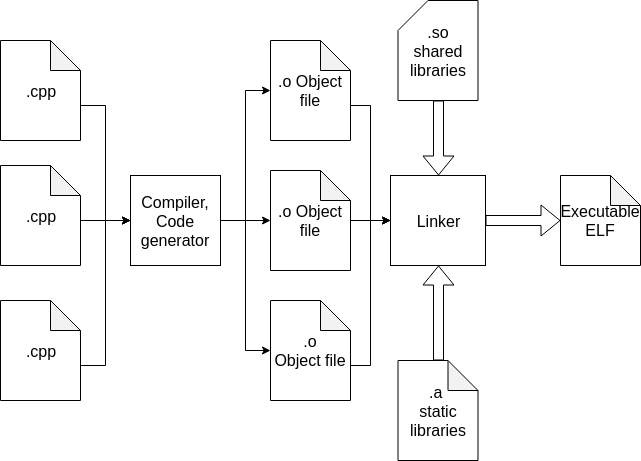
\includegraphics[scale=0.35]{CompilationDiagram.png}
\end{frame}

\begin{frame}
\frametitle{Compilation at a glance}
	\begin{itemize}
		\item \codeinline{.text} - compiled code
		\item \codeinline{.rodata} - variable initialization data + constants + strings
		\item \codeinline{.data} - all global and static variables
		\item \codeinline{.bss} - Better Save Space, zero-initialized variables
	\end{itemize}

	\centering
	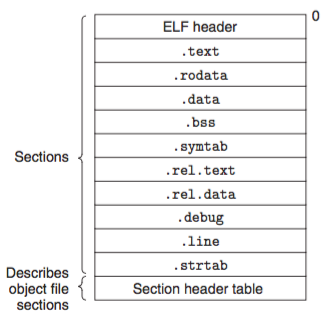
\includegraphics[scale=0.35]{RelocatedObject.png}
\end{frame}

\subsubsection{Compile-time feature toggle}

\begin{frame}[fragile]
\frametitle{\subsubsecname}
\small
\begin{multicols}{2}
main.cpp
\begin{verbatim}
#ifdef FEATURE
class FeatureImpl {
//...	
};

#endif

int main(void) {
#ifdef FEATURE
	registerFeature(new FeatureImpl());
#endif
	//other code...
}
\end{verbatim}

\columnbreak

CMakeLists.txt:
\begin{verbatim}
option(FEATURE "Some feature" ON)
$ cmake .. -DFEATURE=OFF
\end{verbatim}
\end{multicols}
\end{frame}

\subsubsection{Compilation options}

\begin{frame}
\frametitle{\subsubsecname}
\begin{itemize}
	\item \codeinline{-Os} - smaller and (maybe) faster than -O3 
	\item \codeinline{-s} - strip resulting binary object in gcc
	\item \codeinline{-mtune} - use CPU-specific compiler optimizations. Enables usage of extended CPU instruction set
	\item \codeinline{-fno-unroll-loops} - do not unroll loops, may produce less code.
	\item \codeinline{-fno-inline-small-functions} -finline-functions-called-once - optimization of inline functions, inline in certain cases
	\item \codeinline{-fshort-enums} – shrink enums size to max contained value; WARNING: may break ABI (USE ONLY for static binaries)
\end{itemize}
\end{frame}

\subsubsection{Link options}

\begin{frame}
\frametitle{\subsubsecname}
\begin{itemize}
\item \codeinline{-ffunction-sections -fdata-sections -Wl,--gc-sections} - every function and variable goes to its own section, then unused sections are thrown out (up to 30\% improvement)
\item \codeinline{strip --strip-all} on the final executable (up to 20\% improvement)
\item \codeinline{-flto} - LTO, link-time optimization, allows to optimize code across multiple object files
\item \codeinline{strip --remove-section=.comment --remove-section=.note} - removing many copies of garbage strings like "GCC: (GNU) 4.0.1 20050727 (Red Hat 4.0.1-5)"
\end{itemize}
\end{frame}

\subsubsection{Code refactoring}

\begin{frame}
\frametitle{\subsubsecname}
\begin{itemize}
    \item Static vs. dynamic linking
    \begin{itemize} 
    	\item Static libraries: better, if used by one application. 
    	\item Split functions to source files, the resulting binary will be smaller and better optimized (great example: static libc and similar). \\ WARNING: use static linking with caution, since it may cause undefined behavior and program crashes when used incorrectly
    	\item Dynamic libraries: less code size if used by multiple applications
        \item Link only used libraries
	\end{itemize}
\small
\end{itemize}
\end{frame}

\begin{frame}[fragile]
\begin{itemize}
    \item Reasonable logging. Logs often use similar strings:
\begin{verbatim}
$ strings AudioManager
 ...
 DBusWrapper::DBusWrapper DBus Connection is null
 DBusWrapper::DBusWrapper DBus Connection is
 ...
 DBusWrapper::DBusWrapper Registering of watch functions failed
 DBusWrapper::DBusWrapper Registering of timer functions failed
\end{verbatim}
\normalsize
\end{itemize}
\end{frame}

\begin{frame}[fragile]
\frametitle{\subsubsecname}
\begin{itemize}
    \item \codeinline{struct}/\codeinline{class} alignment and packing
    \item Use less C++ templates
    \item Pay attention to \codeinline{inline} functions
    \item Do not use C++ exceptions, compiler option: \codeinline{-fno-exceptions}
    \item Do not use C++ RTTI, compiler option: \codeinline{-fno-rtti}
    \item Statically initialized large arrays and C++ objects with custom (nonzero) data. The initialization data usually goes to \codeinline{.text} block. 
    \small
\begin{verbatim}
    static const std::vector<T> -> static const T[]
    static const std::string -> static const char*
\end{verbatim}
\normalsize
\end{itemize}
\end{frame}

\subsubsection{Compression}

\begin{frame}
\frametitle{\subsubsecname}
\center
\Large UPX \normalsize \\
\url{https://upx.github.io} \\
In-place decompression of compressed executable/library
\end{frame}

\subsubsection{Disable optimization}

\begin{frame}
\frametitle{\subsubsecname}
\begin{itemize}
	\item \codeinline{volatile} keyword
	\item \codeinline{\#pragma GCC optimize("O0")}
\end{itemize}
\end{frame}

\section{Real-life example}
\begin{frame}
\frametitle{\secname}
\center
GENIVI AudioManager \\
\url{https://github.com/GENIVI/AudioManager.git} \\
Intel Core i7, x86-64, Linux, gcc 7.4.0, clang 6.0.0

\end{frame}

\begin{frame}
\frametitle{\secname}

GCC:
\begin{itemize} 
\item \codeinline{cmake .. -DWITH\_CAPI\_WRAPPER=OFF -DWITH\_DBUS\_WRAPPER=ON} 
\item Flags: \codeinline{-fno-unroll-loops -fno-inline-small-functions \\-finline-functions-called-once}
\end{itemize}
Clang: 
\begin{itemize}
\item \codeinline{CC=/usr/bin/clang CXX=/usr/bin/clang++ cmake .. -DCMAKE\_USER\_MAKE\_RULES\_OVERRIDE=\$(pwd)/../ClangDefinitions.txt -DWITH\_CAPI\_WRAPPER=OFF -DWITH\_DBUS\_WRAPPER=ON}
\item Flags: \codeinline{-fvectorize}
\end{itemize}

Libraries are linked statically!
\end{frame}

\begin{frame}[fragile]
\frametitle{\secname}
\center
\begin{table}
\resizebox{\textwidth}{!}{%
\begin{tabular}{|c|c|c|c|c|c|l|l|}
\hline
Release (-O2) & \multicolumn{1}{c}{MinSizeRel (-Os)} & \multicolumn{1}{c}{-march=corei7} & \multicolumn{1}{c}{Section GC flags} & \multicolumn{1}{c}{Misc flags} & \multicolumn{1}{c}{LTO} & \multicolumn{1}{c}{Clang}                                                                          & \multicolumn{1}{c}{gcc}                                                                           \\ \hline
V                                 &                                      &                                   &                                      &                                &                         & \begin{tabular}[l]{@{}l@{}}1020K (not stripped)\\ 780K (stripped)\end{tabular} & \begin{tabular}[l]{@{}l@{}}1.1M (not stripped)\\ 819K (stripped)\end{tabular} \\ \hline
                                  & V                                    &                                   &                                      &                                &                         & \begin{tabular}[l]{@{}l@{}}1.1M (not stripped)\\ 764K (stripped)\end{tabular}  & \begin{tabular}[l]{@{}l@{}}947K (not stripped)\\ 651K (stripped)\end{tabular} \\ \hline
                                  & V                                    & V                                 &                                      &                                &                         & 764K (stripped)                                                                & 651K (stripped)                                                               \\ \hline
                                  & V                                    & V                                 & V                                    &                                &                         & 764K (stripped)                                                                & 651K (stripped)                                                               \\ \hline
                                  & V                                    & V                                 & V                                    & V                              &                         & 764K (stripped)                                                                & 651K (stripped)                                                               \\ \hline
                                  & V                                    &                                   &                                      &                                & V                       & FAILED                                                                         & 499K (stripped)                                                               \\ \hline
                                  & V                                    & V                                 & V                                    & V                              & V                       & FAILED                                                                         & 487K (stripped) \\ \hline                                                              
\end{tabular}%
}
\end{table}
\end{frame}

\section{Further research}

\begin{frame}
\frametitle{\secname}
\begin{itemize}
    \item Yocto tinification on real example
    \item Test on Aarch64 architecture
    \item Run optimization for current Yocto image
    \item Clang LTO + advanced optimization research
\end{itemize}
\end{frame}

\section{Resources}

\begin{frame}
\frametitle{\secname}
\tiny

Executable size reduction techniques in Linux

\begin{itemize}
\item \url{https://wiki.wxwidgets.org/Reducing_Executable_Size}
\item \url{http://www.catch22.net/tuts/win32/reducing-executable-size}
\item \url{http://ptspts.blogspot.com/2013/12/how-to-make-smaller-c-and-c-binaries.html}
\item \url{https://elinux.org/images/0/07/Opdenacker-embedded-linux-size-reduction-techniques.pdf}
\item \url{https://s3-eu-west-1.amazonaws.com/downloads-mips/mips-documentation/login-required/using_gcc_toolchain_options_to_optimize_code_size.pdf}
\item \url{https://medium.com/@aka.rider/how-to-optimize-c-and-c-code-in-2018-bd4f90a72c2b}
\item \url{http://www.muppetlabs.com/~breadbox/software/tiny/teensy.html}
\item \url{http://events17.linuxfoundation.org/sites/events/files/slides/elc14_raj.pdf}
\item \url{https://elinux.org/System_Size\#Hand-optimizing_programs.2C_for_size}
\item \url{https://blog.qt.io/blog/2019/01/02/qt-applications-lto/}
\end{itemize}
\end{frame}

\begin{frame}
\frametitle{\secname}
\tiny

GCC optimization options

\begin{itemize}
\item \url{http://gcc.gnu.org/onlinedocs/gcc/Optimize-Options.html}
\item \url{https://gcc.gnu.org/onlinedocs/gcc/Code-Gen-Options.html}
\item \url{https://gcc.gnu.org/onlinedocs/gcc/C_002b_002b-Dialect-Options.html}
\end{itemize}

Shrinking the linux kernel

\begin{itemize}
\item \url{https://lwn.net/Articles/744507/} - "Shrinking the kernel with link-time optimization"
\item \url{https://lwn.net/Articles/746780/} - "Shrinking the kernel with an axe"
\end{itemize}

Yocto tinification

\begin{itemize}
\item \url{https://elinux.org/images/2/2b/Elce11_hart.pdf}
\item \url{https://elinux.org/images/5/54/Tom.zanussi-elc2014.pdf}
\item \url{https://wiki.yoctoproject.org/wiki/Poky-Tiny}
\end{itemize}
\end{frame}

\begin{frame}
\frametitle{Links}
\small
GENIVI AudioManager fork: \\ \url{https://github.com/alivenets/AudioManager.git}
\newline \newline
Presentation sources: \\ \url{https://github.com/alivenets/binary-footprint-optimize-latex}
\end{frame}

\begin{frame}{}
\center \Huge Thanks for your attention!
\end{frame}

\end{document}
